\chapter{Related Work}
\label{cha:related-work}

\section{Introduction}
Mobile phones, tablets and laptops have become our every day companions. We take them with us wherever we go, may it be the classroom or meetings, lately they have even made an appearance in courtrooms \cite{Farrell:TrialByTablet}. Especially during presentations, mobile device usage is still perceived as rude and can be a source of distraction \cite{Bohmer:SmartphoneUseRude, Bajko:ComparativePerceptionSmartphoneMeeting, Kuznekoff:ImpactPhoneStudentLearning} although other studies indicate that lecture-relevant phone use in classrooms can actually be beneficial \cite{Kuznekoff:MobilePhoneClassroomTwitter}.

Instead of banning modern technologies, incorporating mobile devices into presentation workflows has proven to foster collaboration and connection between attendees in meetings \cite{Bohmer:SmartphoneUseRude} and could possibly promote participation and help introverts overcome the hurdle of speaking out loud \cite{Bry:Backstage}. The growing computing power as well as the ubiquitousness of mobile phones, tablets and laptops make them suitable candidates for giving instant feedback to speakers as well as voting and sharing relevant multi-media content on-the-fly. Resulting presentations provide more flexibility, a better understanding of the listeners' opinion and the potential to close the gap between the presenter and the audience.

In the following, related work is presented to both establish a context for my thesis and set my approach apart from existing ones. In the end the goals of my project and thesis are defined and discussed.

\section{Related work}

The idea of using electronic devices to foster group interaction in meetings is not new. Stefik et al. already experimented with the use of personal computers in meeting rooms as early as in 1987 \cite{Stefik:BeyondTheChalkboard}. Since then, digital whiteboards, telepresence systems, productive multi-user web applications and other computer-aided collaboration tools have become a common sight. The use of portable devices like clickers or mobile phones in presentations, however, is a fairly new field which has only been studied over the last 5 to 10 years.

\subsection{Classroom-related}
Most of this research has been conducted in the educational sector, where growing class-sizes have caused student participation to sink drastically \cite{Bry:Backstage}. The first ap\-proa\-ches in this field of student-response-systems (SRS) utilised so-called clickers -- remote-control-like devices that are connected to a receiver station via radio frequency technology \cite{cuclickers:faq} and can be used for tasks like taking attendance and voting \cite{Chamillard:StudentResponseSystem}. Using these clicker systems -- without grading the students' responses -- has shown to ``yield a strong and positive relationship with student learning'' \cite{Chamillard:StudentResponseSystem}. However, the limitations of clickers -- the need for proprietary hardware and the limited interface consisting only of a few buttons -- lead researchers to experiment with mobile phones as input devices. In 2007 Lindquist et al. presented a system integrated with University of Washington's Classroom Presenter software, which lets students submit answers to assignments and in-class quizzes via SMS and MMS \cite{Lindquist:ExploringMobilePhonesActiveLearning}. Around the same time, the first web-based approaches were explored. Esponda for example describes a system in which iPods and other devices with access to wifi can be used to answer questions during class \cite{Esponda:ElectronicVotingOnTheFly}. What is interesting about her approach is not only the technology used, but also that questions do not have to be prepared in advance, but can also be created on-the-fly, using a pen-based tablet, resulting in more lively and spontaneous student-teacher-interaction.

More recent publications make use of modern web brow\-sers' possibilities to enhance lectures and the interactivity of presentations. The tool \emph{ASQ} \cite{Triglianos:InteractiveWebPresentationsImpress} for example lets lecturers create HTML5 presentations with \emph{impress.js}\footnote{http://impress.github.io/impress.js} which are then distributed to listeners via a link. Students follow the presentations on their mobile devices, and can submit questions connected to the current slide to the speaker. Quizzes (both open questions and multiple-choice) can be embedded in the slides by the teacher, but must be prepared in advance. These quizzes can either be graded automatically (for coding assignments and multiple-choice questions), corrected by teaching assistants or by the students in self or peer-assessment. Another interesting approach is presented by Cheng et al. \cite{Cheng:TreebasedOnlinePresentations}, who propose a system which generates HTML presentations out of \emph{Microsoft PowerPoint} slides and lets viewers add their own content (either additional material or questions) as vertical sub-slides. This way a tree-like structure is created in which teachers and students collaborate in interactive presentations.

Another popular application, with richer audience-spea\-ker-in\-ter\-ac\-tion and an emphasis on listener-listener-interaction is \emph{Backstage} \cite{Bry:Backstage}. As digital backchannels like Twitter can foster the sense of community within the audience, but are usually hard to follow for presenters, Bry et al. developed a backchannel specifically for large classrooms. Students can post messages publicly and send private messages to their colleagues. These public posts can be up or down-voted, as well as marked as unrelated. Together with an ageing-algorithm, this community feedback is used to estimate a post's relevance. Important feedback is then presented to the lecturer, to allow him/her to get a better sense for the audiences' opinion and understanding. Additionally, small quizzes and polls serve as performance feedback to the teacher.

\subsection{Meeting-environments and general approaches}

In contrast to classroom-related software, meeting-en\-vi\-ron\-ments usually have an significantly lower amount of participants, as well as a smaller gap between the speaker and the audience. Another difference lies in the polling, surveying and quizzing functionality which most of the presented projects offer: while these usually have one correct answer in educational settings, to grade students \cite{Lindquist:ExploringMobilePhonesActiveLearning, Triglianos:InteractiveWebPresentationsImpress, Bry:Backstage}, the goal in other environments is to make decisions and collect ideas, without judgment.
One publication which concentrates on these polls and their real-time evaluation and rendering is \cite{Inoue:RealTimeQuestionnaire}: Inoue et al. present a system which distributes \emph{Microsoft PowerPoint} presentations using modern web-technologies while making it possible to alter and update the slides in presentation mode. This way questionnaires can be answered and their results displayed in real-time. Additionally, members of the audience can add annotations (both handwritten and digital) to slides. Although this approach seems very promising, pictures, videos and other types of media are ignored in the project. Moreover the interface seems to complicated to be used on small devices and is therefore only usable on laptops and maybe tablets. Systems designed for multi-device use are proposed in \cite{Bohmer:SmartphoneUseRude} and \cite{Teevan:MobileFeedbackDuringPresentation}. In \cite{Bohmer:SmartphoneUseRude} as well as examining the perception of smartphone use in meetings, the mobile application \emph{Meetster} is presented. The study finds that although people primarily use their phones for meeting or work-related tasks, they tend to think their colleagues use theirs for private purposes. Unlike my work, in which mobile devices should be used in the context of presentations, \emph{Meetster} was developed to help getting to know other meeting attendees in a playful way. This changed the perception of using one's smartphone during the meeting and was described as ``fostering social interactions''.

\begin{figure}
  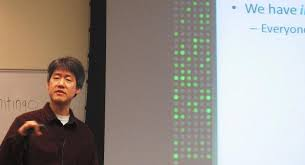
\includegraphics[width=0.9\columnwidth]{figures/feedback-meetings-ms-research}
  \caption{\emph{Crowd Feedback} \cite{Teevan:MobileFeedbackDuringPresentation} used during a presentation. The bar next to the slides shows one dot per participant in the meeting. The feedback dots fade out over time.}
  \label{fig:crowd-feedback}
\end{figure}

\emph{Crowd Feedback} \cite{Teevan:MobileFeedbackDuringPresentation} is a system for displaying continuous, real-time feedback to the speaker in presentations. A responsive web application with a like and dislike button controls the feedback-system. The participants' reactions are shown with a red (dislike) or green (like) dot for each attendee in a sidebar next to the presentation slides. An evaluation of the system showed that the participants felt more engaged with the presentation and connected to other listeners. Many users stated only having the possibility to like or dislike did not reflect enough options and that a button related to the speech pace might have helped. It was also noted that the sidebar was perceived as disturbing and made it harder to pay close attention to the presentation.

\section{Goals}
The main aim of the project and thesis is to explore different ways of incorporating mobile devices into presentations in business-settings efficiently and productively. This includes polls created by the speaker (both beforehand and on-the-fly), as covered by other studies, as well as continuous, spontaneous feedback as described in \cite{Teevan:MobileFeedbackDuringPresentation}. Additionally other types of annotations should be supported, namely textual comments, images, links and youtube-videos, which will be rendered accordingly on new presentation slides. I believe this approach has the potential of transforming presentations into an collaborative effort in which all meeting-participants are empowered to shape the progress and outcome of presentations. From a technological point of view, like most existing approaches \cite{Bry:Backstage, Cheng:TreebasedOnlinePresentations, Esponda:ElectronicVotingOnTheFly, Inoue:RealTimeQuestionnaire, Teevan:MobileFeedbackDuringPresentation, Triglianos:InteractiveWebPresentationsImpress}, an web application will be developed to make use of modern web technologies' quick prototyping capabilities and the web's cross-platform and cross-device nature. As \emph{WebSockets} have successfully been deployed in the real-time features of other presentation tools \cite{Inoue:RealTimeQuestionnaire, Triglianos:InteractiveWebPresentationsImpress} (in \cite{Inoue:RealTimeQuestionnaire} a difference in response time between 10 and 600 simultaneous users of under 150ms and a package loss of approximately 0\% was reported), this technology will be used to communicate between speaker and audience. Like in \cite{Triglianos:InteractiveWebPresentationsImpress}, an existing web presentation library will be used to be able to concentrate on the collaborative features rather than building a cross-device presentation platform. Instead of \emph{impress.js}, \emph{reveal.js}\footnote{http://lab.hakim.se/reveal-js/} will be used for this purpose, as it already offers a few key features, namely focus on mobile devices, embedded videos, speaker-notes and a possibility to follow or control presentation from ones personal device.